% FedAuditor -- IEEE conference paper (6 pages).
% Build from this folder: pdflatex fedauditor; bibtex fedauditor; pdflatex fedauditor; pdflatex fedauditor
% Tables come from `python -m fedauditor.make_figures` (run in Final-Year/) and are \input from
% ../results/fedauditor/figures/, so re-running the script keeps the paper in sync with the results.
\documentclass[conference]{IEEEtran}
\usepackage[utf8]{inputenc}
\usepackage[T1]{fontenc}
\usepackage{amsmath,amssymb}
\usepackage{booktabs}
\usepackage[table]{xcolor}
\usepackage{graphicx}
\usepackage{textcomp}
\usepackage{tikz}
\usetikzlibrary{positioning,arrows.meta,fit}
\usepackage{url}
\usepackage[hidelinks]{hyperref}

\newcommand{\figdir}{../results/fedauditor/figures}

\begin{document}

\title{FedAuditor: Auditing Federated Clinical Models with a Privacy-Budgeted, Fact-Checked LLM Agent}

\author{\IEEEauthorblockN{Author One\IEEEauthorrefmark{1}, Author Two\IEEEauthorrefmark{1}, Author Three\IEEEauthorrefmark{2}}
\IEEEauthorblockA{\IEEEauthorrefmark{1}Department, Institution, City, Country}
\IEEEauthorblockA{\IEEEauthorrefmark{2}Department, Institution, City, Country\\
\{author.one, author.two\}@institution.edu}}

\maketitle

\begin{abstract}
Federated learning lets hospitals and health agencies train a shared model without moving patient
records, but it also takes the data away from the people who must decide whether that model can be
trusted. One site with mislabelled outcomes, a broken export or an under-diagnosed subgroup can
change what the model learns, while pooled accuracy stays where it was. We ask whether a large
language model (LLM) agent can do this kind of audit when it is only allowed to see what a careful
coordinator would see. FedAuditor gives the agent eight aggregate tools; every tool adds Laplace
noise, charges a fixed privacy budget and logs its output, and every number in the agent's final
report must point to a logged value that a deterministic fact-checker can find. We also release
FedFault, a benchmark that plants eight kinds of fault at three severities in a 52-client federation
built from the 2023 BRFSS survey, with each US state or territory acting as one client. Over 125
held-out scenarios with logistic regression, Claude Haiku~5.5 found the faulty clients with
precision 0.97 and recall 0.89 and named the fault correctly in 91\% of scenarios, compared with
0.99, 0.88 and 87\% for a tuned rule-based auditor using the same tools and budget. The agent was
much better at subgroup bias, worse at faint drift, and 2{,}262 of its 2{,}264 numeric claims were
verified. The full evaluation cost US\$1.16.
\end{abstract}

\begin{IEEEkeywords}
federated learning, model auditing, LLM agents, differential privacy, clinical prediction, diabetes
\end{IEEEkeywords}

% ================================================================================================
\section{Introduction}

Federated averaging~\cite{mcmahan2017fedavg} is now a familiar answer to a familiar problem in
health informatics: the data needed to train a good model sit in many institutions that cannot
share them~\cite{rieke2020future,kairouz2021advances}. Each site trains locally and sends back a
model update, and a coordinator averages the updates. Nobody pools the records.

This arrangement has a side effect that gets less attention. The coordinator is usually the party
asked to vouch for the model, yet it is the one party that never sees the data. If a regional
registry starts exporting missing body-mass values as zero, or if one site's positives in a
particular subgroup are systematically coded as negative, the coordinator has no direct way to
notice. Pooled metrics do not help much. In our benchmark, seven of the eight planted fault types
move pooled test AUC by at most 0.001, which is smaller than the 0.008 that AUC varies between clean
runs with different seeds (Table~\ref{tab:pooled}). Only aggressive model poisoning shows up.

Finding such faults is investigative work. An auditor has to look across many sites, spot the one
statistic that is out of line, rule out look-alike explanations and estimate when the problem
began. That is the kind of open-ended, tool-driven task where LLM agents~\cite{yao2023react,
schick2023toolformer} are starting to be useful. Two obstacles stand in the way, though. First, an
agent with broad data access becomes a new privacy risk, which defeats the purpose of federating in
the first place. Second, LLMs are known to state numbers that were never in their
input~\cite{ji2023hallucination}, and an audit report with an invented statistic is worse than no
report.

FedAuditor is our attempt to remove both obstacles by construction. The agent never touches a
record: it can only call tools that compute statistics at the clients, add calibrated Laplace
noise~\cite{dwork2006calibrating} and charge a per-audit privacy budget. Its report is structured,
and every finding is backed by claims of the form \emph{(tool call, metric, value, keys)} that a
fact-checker looks up in the tool log. A claim that cannot be found is flagged, not trusted.

We make four contributions:
\begin{itemize}
\item \textbf{FedFault}, a benchmark of eight planted faults (label noise, covariate drift, update
  poisoning, free-riding, prevalence shift, subgroup under-diagnosis, a missing-data artefact and
  explanation instability) at three severities and five seeds, with clean runs for false alarms, on
  a 52-client BRFSS federation and three model families.
\item \textbf{Noise-aware, privacy-budgeted audit tools} that wrap an existing federated measurement
  layer and report outlier scores that account for each client's own noise level.
\item \textbf{A claim-level fact-checker}, plus a dashboard that links every claim to the logged row
  it cites.
\item \textbf{An evaluation} against a tuned rule baseline with the same tools and budget, including
  a prompt ablation, per-fault results, cost, and the failure modes of two open-weight models.
\end{itemize}

% ================================================================================================
\section{Related Work}

\textbf{Robustness and attacks in FL.} A large body of work protects aggregation against bad
updates, for example Krum~\cite{blanchard2017krum} and coordinate-wise median or trimmed
mean~\cite{yin2018byzantine}, and studies the attacks themselves: backdoors~\cite{bagdasaryan2020backdoor},
sybils~\cite{fung2020sybil} and free-riders~\cite{fraboni2021freerider}. These methods are designed
to defend the aggregate automatically against one threat. They do not explain what went wrong, and
most of them only look at update vectors, so data-level faults such as a subgroup coding error are
out of scope.

\textbf{Detecting data problems.} Dataset-shift detection~\cite{rabanser2019failing},
calibration checks~\cite{vancalster2019calibration} and subgroup audits~\cite{obermeyer2019dissecting}
are standard in centralised clinical ML. Feature attributions~\cite{lundberg2017shap} and data
valuation~\cite{ghorbani2019shapley} are used to see what a model relies on and who contributed.
The original FedHealth system we build on already computed federated versions of several of these
measurements; FedAuditor turns them into tools that an agent can call under a budget.

\textbf{Agents for federated learning.} Several recent systems use LLM agents inside FL.
FedAgentBench~\cite{saha2025fedagentbench} tests whether agents can set up federated medical imaging
pipelines, Agentic-FL~\cite{jarczewski2026agentic} argues for agents as orchestrators of training,
and FL-MAESTRO~\cite{wu2026flmaestro} lets specialist agents choose topology, aggregation and
resources every round. All of them use agents to \emph{run} federated training. None of them asks
whether the resulting model is sound.

\textbf{Agents that audit models.} ModelAuditor~\cite{kuhn2025modelauditor} is the closest work in
spirit: an agent that audits a clinical imaging model by simulating distribution shifts and
reporting on robustness. It assumes direct access to the model and an in-distribution dataset. Our
setting is federated and the agent has neither, which changes both the tools and the evaluation.

\textbf{Grounded generation.} Methods that make LLM output checkable, such as generating text with
citations~\cite{gao2023alce} or scoring atomic facts against a source~\cite{min2023factscore}, inspired
our report format. Because our evidence is a structured tool log rather than free text, the check can
be exact and does not need a second model.

% ================================================================================================
\section{Problem Setting}

A coordinator runs $R$ rounds of FedAvg over $K$ clients. Client $k$ holds $n_k$ records split into
train, calibration and test parts. After training, an auditor must return a list of findings, each
naming a client, one of the eight fault types, an onset round and a confidence. The auditor may
not read records, labels or raw updates. It may only ask for aggregate statistics, which the
clients compute locally and release with noise. Each audit has a privacy budget $\varepsilon_{\max}$;
once it is spent, further queries are refused. We treat the clients as honest but possibly faulty:
a fault may be accidental (an export bug) or deliberate (poisoning), but clients answer audit
queries truthfully. Collusion between a faulty client and the audit tools is out of scope.

% ================================================================================================
\section{The FedFault Benchmark}

\textbf{Data.} We use the 2023 Behavioral Risk Factor Surveillance System~\cite{cdc2023brfss},
recoded to predict self-reported diabetes from standard risk factors (blood pressure, cholesterol,
BMI, smoking, activity, general and physical health days, age group, sex, income and others). After
removing incomplete cases we keep about 291{,}000 respondents with 13.6\% prevalence. Each of the 52
states and territories becomes one client, so client sizes vary widely; the smallest, Guam, has
1{,}182 records. Imputation and feature scaling are computed federatively.

\textbf{Models.} Training uses Flower~\cite{beutel2020flower} for 20 rounds of FedAvg with logistic
regression (LR) and a small MLP, and tree bagging for XGBoost~\cite{chen2016xgboost}. On clean data
federated training matches central training: pooled AUC is 0.821 vs 0.821 for LR, 0.826 vs 0.826 for
XGBoost and 0.816 vs 0.828 for the MLP, which is still improving at round 20. Per-state AUC ranges
from 0.76 to 0.87.

\textbf{Faults.} Each scenario plants one fault in three clients (about 5\% of the federation),
chosen among clients with at least median training size. The same three clients are used at every
severity for a given seed, so severities can be compared directly. The severities (low/medium/high)
are:
\emph{label noise}, fraction of labels flipped (0.1/0.2/0.3);
\emph{drift}, the three features most correlated with the outcome shift by $k$ standard deviations
from mid-training (0.5/1/2);
\emph{poisoning}, the update is replaced by $-k$ times itself (1/3/10);
\emph{free-riding}, fraction of rounds in which the client returns the global model with tiny noise
instead of training (0.3/0.6/1.0);
\emph{prevalence shift}, only $1/k$ of negatives are kept (2/4/8);
\emph{subgroup bias}, fraction of positives in one subgroup recorded as negative (0.3/0.6/0.9);
\emph{missing-data artefact}, fraction of rows in which two features are exported as a sentinel code
instead of missing (0.1/0.25/0.5); and
\emph{explanation instability}, noise of $k$ times the update's own norm added to every upload
(1/3/10), which leaves accuracy alone but makes feature attributions jitter from round to round.
The ground truth stores the affected clients, the onset round and the fault parameters.

\input{\figdir/pooled_auc.tex}

Table~\ref{tab:pooled} shows why these faults are worth auditing for. Apart from high-severity
poisoning, which lowers pooled AUC by 0.184 for LR and 0.207 for the MLP, no fault moves pooled AUC by
more than 0.001 on average. A monitoring dashboard built on pooled performance would report all of
them as healthy.

\textbf{Protocol and scoring.} Seed 10 is reserved for development: writing prompts and tuning the
baseline. Evaluation uses seeds 20 to 24, giving $8 \times 3 \times 5 = 120$ faulty scenarios and 5
clean ones per model. Precision and recall are computed over clients and micro-averaged across
faulty scenarios. Type accuracy counts a scenario as correct when the most frequently reported fault
type is the planted one (a tie among $k$ types earns $1/k$). Onset error is the mean absolute error
in rounds over correctly flagged clients, and the false-alarm rate (FAR) is the share of clean runs
with at least one finding.

% ================================================================================================
\section{FedAuditor}

Fig.~\ref{fig:arch} shows the pipeline. The parts that matter most are the tools, the budget, the
report format and the fact-checker.

\begin{figure}[t]
\centering
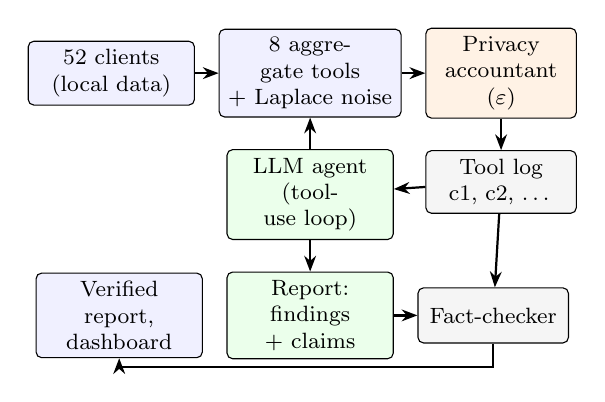
\begin{tikzpicture}[font=\footnotesize, node distance=4mm and 3mm,
  box/.style={draw, rounded corners=2pt, align=center, inner sep=3pt, minimum height=7mm},
  arr/.style={-{Stealth[length=2mm]}, thick}]
\node[box, fill=blue!6, text width=19mm] (fed) {52 clients\\(local data)};
\node[box, fill=blue!6, text width=21mm, right=of fed] (tools) {8 aggregate tools\\+ Laplace noise};
\node[box, fill=orange!10, text width=17mm, right=of tools] (acct) {Privacy\\accountant ($\varepsilon$)};
\node[box, fill=green!8, text width=19mm, below=of tools] (agent) {LLM agent\\(tool-use loop)};
\node[box, fill=gray!8, text width=17mm, below=of acct] (log) {Tool log\\c1, c2, \ldots};
\node[box, fill=green!8, text width=19mm, below=of agent] (report) {Report: findings\\+ claims};
\node[box, fill=gray!8, text width=17mm, right=of report] (fc) {Fact-checker};
\node[box, fill=blue!6, text width=19mm, left=of report] (dash) {Verified report,\\dashboard};
\draw[arr] (fed) -- (tools);
\draw[arr] (tools) -- (acct);
\draw[arr] (agent.north) -- (tools.south);
\draw[arr] (acct) -- (log);
\draw[arr] (log) -- (agent);
\draw[arr] (agent) -- (report);
\draw[arr] (report) -- (fc);
\draw[arr] (log) -- (fc);
\draw[arr] (fc.south) |- ++(0,-3mm) -| (dash.south);
\end{tikzpicture}
\caption{FedAuditor. The agent only sees noisy aggregates released through budgeted tools. Every
call is logged, and each claim in the final report is checked against that log.}
\label{fig:arch}
\end{figure}

\subsection{Privacy-budgeted tools}

The agent can call eight tools. \texttt{federation\_overview} is free and lists the clients with their
sizes, the features and the sensitive attributes. The other seven cost budget:
\texttt{global\_performance}; \texttt{client\_performance} (AUC, ECE, Brier score, prevalence, mean
prediction and calibration-in-the-large per client); \texttt{client\_updates} (each client's update
norm relative to the median and its cosine similarity to the median update, overall or per round);
\texttt{feature\_summary} (mean, standard deviation and 1st/99th percentiles in raw units);
\texttt{subgroup\_outcomes} (observed-to-expected ratio and false-negative rate per subgroup);
\texttt{drift\_by\_round} (feature shift, estimated onset and calibration drift); and
\texttt{attribution\_churn}. Statistics are computed at the clients by the measurement modules of
the original system, and only compact tables leave the client.

If a call releases $m$ statistics per client and is given budget $\varepsilon$, each statistic
receives Laplace noise with scale $c\,m/(n\varepsilon)$, where $n$ is the number of records behind
the statistic and $c$ is its range after clipping (features are clipped at $\pm 8$ standard
deviations of the federation mean). A call costs 1 by default, the agent may spend more on a call to
get less noise, and each audit has $\varepsilon_{\max} = 20$. A \texttt{PrivacyAccountant} charges
each call, refuses calls once the budget is gone and refunds calls that fail. Clients see disjoint
records, so a single call is charged once rather than once per client.

\textbf{Noise-aware flags.} Since noise scales with $1/n$, a naive outlier rule will keep pointing
at the smallest states. Each client table therefore includes a \texttt{flags} column that lists the
statistics whose noise-adjusted score
\begin{equation}
z_k = \frac{v_k - \operatorname{median}_j(v_j)}{\sqrt{s^2 + \sigma_k^2}}
\end{equation}
exceeds 3 in absolute value, where $s$ is a robust (MAD-based) spread across clients and $\sigma_k$
the standard deviation of the noise added to client $k$. Update norms grow with client size
(correlation 0.75 in clean runs), so their flags are computed after adjusting for $n_k$. The flags
are post-processing of already released values, so they cost no budget.

\subsection{Agent and report format}

The agent is a standard tool-use loop around an LLM. The system prompt describes the noise model,
tells the agent to screen all clients before drilling into any one of them, maps each tool to the
faults it can reveal and explains how to separate faults that look alike. For instance, label noise
and poisoning both produce updates that point away from the rest, but only label noise lowers the
client's own AUC. The prompt also warns that with 52 clients a score of 3 to 5 should be treated as
a lead rather than a finding. We call this version prompt v5; prompt v4 lacked the paragraphs on
look-alike faults and multiple comparisons.

The final report is JSON with a short summary and a list of findings. Each finding has a client,
fault type, onset round, confidence, a rationale in prose and a list of claims. A claim names a call
id, a metric and a value, and optionally the client, round, feature and group it refers to.

\subsection{Fact-checker}

For each claim the checker retrieves the cited call, rejects it if the call failed, and scans the
call's tables for a row whose key columns match the claim and whose metric lies within
$0.005 + 2\%$ of the claimed value. A cited flag is written as \texttt{<stat>\_z}. Rejected claims are
reported with a reason: unknown call, no matching row, or a value mismatch together with the
closest logged value. The checker is deterministic and costs nothing to run. The dashboard uses the
same matching rule to link each claim to the exact row it came from.

\subsection{Rule baseline}

To tell apart what the agent contributes from what the tools contribute, we wrote a rule-based
auditor with the same tools, budget and report format. It follows a fixed query plan and applies
noise-aware robust thresholds for each fault type. Its thresholds were tuned on the development
seed only; an earlier version that ignored client noise raised false alarms in 3 or 4 of 5 clean runs
because of the small territories.

% ================================================================================================
\section{Experiments}

We ran the rule baseline on all three models and Claude Haiku~5.5 on LR, which was what our API
budget allowed. Each audit is independent: the agent starts with an empty context, a fresh budget
and the free overview. Haiku was run with both prompts on the same 125 scenarios.

\input{\figdir/main_table.tex}
\input{\figdir/type_confusion.tex}

\subsection{Overall results}

Table~\ref{tab:main} gives the main comparison. With prompt v5 the agent and the rules find the
faulty clients about equally well (precision 0.97 vs 0.99, recall 0.89 vs 0.88). The agent names
the fault correctly more often (0.91 vs 0.87) and dates it more precisely (0.24 vs 0.35 rounds). It
raised false alarms in two of the five clean runs, both times flagging Guam at confidence exactly
0.5. Dropping findings at or below that confidence removes both alarms and gives precision 1.00, at
the cost of recall (0.84). We chose that cut-off after looking at the results, so it should be read
as a sensitivity check and not as a tuned operating point.

\input{\figdir/recall_heatmap.tex}

\subsection{Which faults each auditor finds}

Table~\ref{tab:recall} splits recall by fault and severity. Label noise, poisoning, free-riding at
medium and high severity and the missing-data artefact are found almost every time by both
auditors. The clearest difference is subgroup bias: at medium severity the agent finds every
affected client, while the rules find 60\%. Detecting it requires putting together a subgroup query
and the client screen, and the fixed plan only covers part of that space. The agent also does better
on medium explanation instability (1.00 vs 0.87). It does worse on low-severity drift (0.60 vs 0.87)
and low-severity free-riding (0.87 vs 1.00). In both cases the signal is a small but steady
deviation; a threshold catches it reliably, whereas the agent, having been told to be wary of
multiple comparisons, seems to discount it. Neither auditor detects the lowest severity of subgroup
bias (0.13) or explanation instability (0.00). At that level the effect is smaller than the noise
the budget imposes, so this is a limit of the tools rather than of either auditor.

\subsection{Telling faults apart}

The prompt ablation in Table~\ref{tab:confusion} was the largest single improvement we made. With
prompt v4 the agent labelled 12 of the 15 label-noise scenarios as poisoning. Prompt v5 adds a short
paragraph asking the agent to check the client's local AUC before choosing between the two, and all
15 are then typed correctly. Overall type accuracy rose from 0.79 to 0.91 while detection stayed the
same. Every remaining typing error is at low severity. In explanation instability (5 scenarios) and
subgroup bias (4) the agent mostly reports nothing (6 of 9), twice reports Guam as a prevalence
shift, and once flags a correct client but calls the fault poisoning.

\input{\figdir/behaviour.tex}

\subsection{How the agent spends its budget}

Table~\ref{tab:behaviour} summarises audit behaviour. The agent uses the whole budget in almost every
audit, makes about 11.5 calls over 5 turns and finishes in about a minute. The rule baseline makes 8.4
calls and leaves some budget unused. The agent's reports are far more detailed, with 18.1 claims per
audit against 3.6 for the rules. Across the 125 v5 audits, \texttt{subgroup\_outcomes} was the most
used tool (409 calls, in every audit), followed by \texttt{client\_updates} (338),
\texttt{drift\_by\_round} (216), \texttt{feature\_summary} (187) and \texttt{client\_performance}
(136). \texttt{attribution\_churn} was used in only 29 audits, and \texttt{global\_performance} was
never called, which matches the finding that pooled numbers carry little information here.

The fact-checker rejected 9 claims in the v4 audits and 2 in the v5 audits. Most rejections were
malformed metric names (for example \texttt{z} instead of a named flag), but two v4 claims stated
wrong numbers: an observed-to-expected ratio of 7.38 where the log said 1.81, and 1.08 where it said
0.53. Neither error changed which client was flagged, but both would have gone unnoticed in a
free-text report. Each audit cost just under one US cent.

\subsection{Other models}

The rule baseline transfers to the MLP and XGBoost without retuning (Table~\ref{tab:models}), with
precision of at least 0.99 and no false alarms. Recall is lower for XGBoost (0.84), probably because
tree updates are summarised through margins on synthetic probe points, which blurs the update-based
signals. In a single pilot audit of a low-severity poisoning scenario, Claude Opus~5.5 found all three
poisoned clients with 7 of 7 claims verified, for about US\$0.31. We did not run LLM audits on the
other models at scale.

\input{\figdir/rules_models.tex}

\subsection{A worked example}

Table~\ref{tab:example} shows part of one report. In the high-severity subgroup-bias scenario of seed
20, positives among men (\texttt{Sex}$=1$) in Massachusetts, Michigan and Wisconsin were mostly
recorded as negative. The agent screened all clients with five tools, queried subgroup outcomes for
each sensitive attribute and checked the per-round updates of two clients, all within 10 calls and 4
turns. It flagged exactly the three affected states as subgroup bias from round 1, and all 25 of its
claims were verified. In its summary it also listed the leads it decided not to report, such as
update-norm outliers in Guam and Alabama and a feature shift with $z = 3.4$ in Michigan, which is the
behaviour prompt v5 asks for.

\begin{table}[t]
\centering
\footnotesize
\setlength{\tabcolsep}{3pt}
\caption{Claims behind the finding ``MA: subgroup bias, onset round 1, confidence 0.8''. Every value
was found in the cited row of the tool log.}
\label{tab:example}
\begin{tabular}{llrl}
\toprule
Keys & Metric & Value & Cited call \\
\midrule
Sex $=1$ & O/E ratio & 0.000 & c6 \texttt{subgroup\_outcomes} \\
Sex $=1$ & $z_\text{noise}$ & $-8.98$ & c6 \texttt{subgroup\_outcomes} \\
round 20 & prevalence & 0.053 & c3 \texttt{client\_performance} \\
round 20 & mean prediction & 0.102 & c3 \texttt{client\_performance} \\
round 20 & calib.-in-the-large & 0.049 & c3 \texttt{client\_performance} \\
-- & median norm ratio & 3.07 & c2 \texttt{client\_updates} \\
-- & mean cosine & 0.027 & c2 \texttt{client\_updates} \\
\bottomrule
\end{tabular}
\end{table}

\subsection{Open-weight models}

We also wanted to know whether a model that can run on-site would do. Using the same tools and
prompt, we tried three Qwen3 models~\cite{yang2025qwen3} on development scenarios, served locally.
Qwen3-8B fixed its attention on the smallest state and never screened the federation.
Qwen3-30B-A3B in thinking mode needed 16 to 29 minutes per audit and treated noise as faults. The
instruction-tuned Qwen3-30B-A3B-2507 was fast (2 to 3 minutes per audit) and did catch poisoning,
but it kept reporting states with $|z|$ between 3 and 4 despite the warning in the prompt, and it
mis-cited numbers, which the fact-checker caught. Because Haiku succeeded with exactly the same tools
and prompt, we attribute these failures to the models. We did not run these models on the full grid,
so we report them as qualitative observations.

% ================================================================================================
\section{Discussion}

\textbf{What the agent adds.} On aggregate detection scores the agent and a carefully tuned rule
set are close. The agent's advantage shows up where a fixed plan is weakest: faults that only appear
when the right subgroup is queried, and the step of choosing between explanations. It also writes a
report that a clinician or data steward can read, in which every number can be traced. The rule
baseline, in turn, is free, fast and better at faint, steady deviations. In practice the two are
complementary, and running the rules first as a cheap screen before an agent audit is a natural
deployment.

\textbf{What the fact-checker does and does not prove.} The checker guarantees that the numbers in
a report exist in the log. It does not guarantee that the prose interprets them correctly. In the
worked example the agent described the \texttt{Sex}$=1$ subgroup as women, although the BRFSS
recoding uses 1 for men. All of its numbers were right and so was the finding, but the sentence was
wrong. Returning value labels from the overview tool would prevent this particular mistake, and
checking qualitative statements more generally is an open problem.

\textbf{The cost of privacy.} The lowest severities of subgroup bias and explanation instability
were missed by both auditors, and the smallest client caused every false alarm. Both are direct
effects of noise that scales with $1/n$. A larger budget or pooling small territories into one
client would help, at a privacy cost that a real deployment would have to decide on.

% ================================================================================================
\section{Limitations}

Our privacy accounting uses basic composition with a sensitivity of $c/n$, which is exact for means
and rates but only a heuristic for AUC, ECE, quantiles and update statistics; the budget should be
read as a calibrated accounting device, not a formal differential privacy
guarantee~\cite{dwork2014algorithmic,abadi2016dpsgd}. The LLM evaluation covers one dataset and one
model family with five seeds per cell, and only five clean runs, so false-alarm rates are coarse.
The planted faults have a single cause and a clean onset, whereas real federations may suffer from
several overlapping problems. Finally, the clients are assumed to answer audit queries honestly.

% ================================================================================================
\section{Conclusion}

FedAuditor shows that an LLM agent can audit a federated clinical model through noisy, budgeted
aggregates alone, match a tuned rule baseline at finding faulty sites, do better at subgroup bias and
at naming the fault, and back almost every number it reports with a logged tool result, for about a
cent per audit. We plan to release FedFault, the tools and the fact-checker with the code. Next we plan to
replace the heuristic budget with a formal mechanism, run the agent on the MLP and XGBoost
federations, add a second dataset from intensive care, and extend the checker to qualitative claims.

\bibliographystyle{IEEEtran}
\bibliography{refs}

\end{document}
